\section{Zielsetzung}

\noindent
In diesem Versuch wird der Operationsverstärker näher betrachtet. Dazu werden Anwendungsbeispiele eines Operationsverstärkers in Schaltungen realisiert 
und auf ihre Eigenschaften untersucht. Insbesondere werden die Unterschiede eines realen und eines idealen Operationsverstärker aufgezeigt. 

\section{Theorie}

    \noindent
    Es werden im folgenden Abschnitt die theoretischen Grundlagen von Operationsverstärkern dargelegt. 

    \subsection{Eigenschaften}

        \noindent 
        Ein Operationsverstärker ist ein Differenzenverstärker. Das bedeutet, dass die Ausgangsspannung proportional ist zu der Differenz der beiden 
        eingehenden Spannungen 
        \begin{equation*}
            U_\text{A} = V \cdot \left( U_\text{P} - U_\text{N}\right)\, .
        \end{equation*}
        Die Ausgangsspannung ist damit in der Phase von $U_\text{P}$, welche am positiven, nicht-invertierten Eingang liegt ($+$), und gegenphasig zur 
        Spannung $U_\text{N}$, welche am invertierten Eingang ($-$) liegt. Dies ist in \autoref{fig:schaltung} in einem Schaltbild dargestellt. 
        Das dreieckige Symbol ist mittlerweile veraltet, das neue Symbol ist ein Rechteck, wie es in den nachfolgenden Schaltungen zu sehen ist. 
        \begin{figure}%
            \centering%
            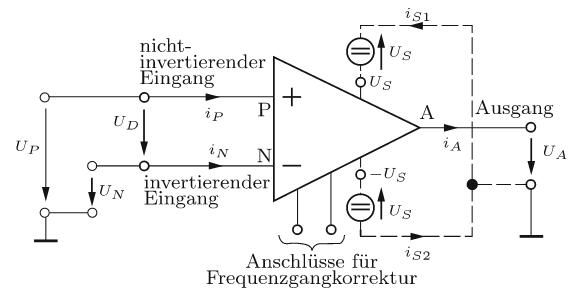
\includegraphics[width=0.8\textwidth]{images/schaltbild_buch.png}%
            \caption{Die Schaltung eines Operationsverstärkers. Die Betriebsspannung $U_\text{B}$ wird normalerweise nicht eingezeichnet. \cite{BrabetzHaasSpieker+2015}}%
            \label{fig:schaltung}%
        \end{figure}%
        Die Proportionalität der Ausgangsspannung zur Differenz der Eingangsspannungen gilt nur für 
        \begin{equation*}
            - U_\text{S} < U_\text{A} < U_\text{S}\, ,
        \end{equation*}
        außerhalb von diesem Bereich ist die Ausgangsspannung entsprechend $\pm U_\text{S}$. Dies ist visuell dargestellt in \autoref{fig:kennlinie}.
        \begin{figure}%
            \centering%
            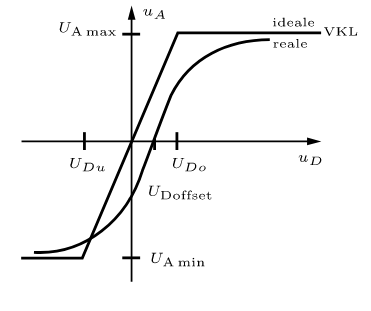
\includegraphics[width=0.4\textwidth]{images/kennlinie_buch.png}%
            \caption{Die Kennlinie eines idealen und eines realen Operationsverstärker. \cite{BrabetzHaasSpieker+2015}}%
            \label{fig:kennlinie}%
        \end{figure}%
        In \autoref{fig:kennlinie} ist bei der Kennlinie des idealen Operationsverstärker zu sehen, dass die die Ausgangsspannung $U_\text{A}$ linear 
        mit der Eingangsspannungsdifferenz $U_\text{D}$ geht in dem Bereich, wo die Bedingung $- U_\text{S} < U_\text{A} < U_\text{S}$ gilt. 
        Die Spannungsdifferenzen, bei denen diese Sättigung einsetzt, werden $U_\text{Du}$ und $U_\text{Do}$ genannt. \\
        Hier in der Abbildung werden Unterschiede zwischen einem idealen und einem realen Operationsverstärkern aufgewiesen. 
        Bei einem idealen Operationsverstärker beträgt die Leerlaufverstärkung $V = \infty$, die Eingangswiderstände $r_\text{e,p}$ und $r_\text{e,n}$ sind hierbei auch unendlich 
        groß, damit in dem Operationsverstärker kein Strom fließt. 
        Der Ausgangswiderstand $r_\text{A}$ ist dabei gleich $0$. Die Übertragungsbandbreite geht von $0$ bis $\infty$, es findet keine Phasendrehung statt. \\ 
        Im Gegensatz dazu hat ein realer Operationsverstärker eine Leerlaufverstärkung von $V \propto 10^4$-$10^6$. 
        Die Eingangswiderstände sind nicht unendlich groß, aber üblicherweise größer als $\SI{1}{\mega\ohm}$. 
        Der Ausgangswiderstand ist im Bereich von $\SI{10}{\ohm}$ - $\SI{1000}{\ohm}$. 
        Die Übertragungsbandbreite hat eine obere Grenze, die sich im Bereich von $\SI{10}{\hertz}$ bis $\SI{10}{\kilo\hertz}$ liegt.
        Es tritt eine Phasendrehung auf. \\
        Aus den Unterschieden des realen Operationsverstärker zu einem Idealen, folgen nur geringe Unterschiede, die kleine Korrekturen in den Rechnungen fordern. 
        Jedoch treten ein paar Phänomene auf, die im folgenden Abschnitt besprochen werden. \\

        \noindent 
        Falls an beiden Eingängen die gleiche Spannung $U_\text{Gl}$ anliegt, sollte es bei einem idealen Operationsverstärker zu einer Ausgangsspannung $U_\text{A} = \SI{0}{\volt}$ 
        kommen, bei einem realen misst man aber die Ausgangsspannung $\increment U_\text{A}$. 
        Dieses Phänomen wird Gleichtaktverstärkung genannt und parametrisiert durch 
        \begin{equation*}
            V_\text{Gl} = \frac{\increment U_\text{A}}{U_\text{Gl}}\, .
        \end{equation*}
        Zudem ist eine Offsetspannung zu messen, da eine Ausgangsspannung zu messen ist, falls beide Eingangsspannungen $0$ betragen. Die Offsetspannung $U_0$ ist als 
        \begin{equation*}
            U_0 = U_\text{P} - U_\text{N}
        \end{equation*}
        definiert, 
        wobei die Eingangsspannungen so gewählt sind, dass $U_\text{A}=0$ gilt. \\
        Dadurch, dass es bei einem realen Operationsverstärker zu endlichen Eingangswiderständen kommt, gibt es einen endlichen Eingangsruhestrom 
        \begin{equation*}
            I_\text{B} = \frac{1}{2}\left( I_\text{P} + I_\text{N}\right)\, .
        \end{equation*}
        Analog lässt sich ein Offsetstrom $I_0$ definieren, 
        \begin{equation*}
            I_0 = I_\text{P} - I_\text{N}\quad \text{bei}\, U_\text{P} = U_\text{N}=0\, .
        \end{equation*}
        Abschließend sind die Differenzwiderstände
        \begin{equation*}
            r_\text{P} = \begin{cases}
                \frac{\increment U_\text{P}}{\increment I_\text{P}} , & U_\text{N}=0\\
                \frac{\increment U_\text{N}}{\increment I_\text{N}} , & U_\text{P}=0
            \end{cases}\, ,
        \end{equation*}
        und der Gleichtakteingangswiderstand 
        \begin{equation*}
            r_\text{Gl} = \frac{U_\text{Gl}}{I_\text{Gl}}
        \end{equation*}
        zu nennen. \\
        Durch diese Phänomene ist die leicht unterschiedliche Kennlinie in \autoref{fig:kennlinie} zu erklären. 

    \subsection{Schaltbeispiele mit Operationsverstärkern}

        \noindent 
        Im folgenden Abschnitt werden die im Versuch genutzten Schaltungen vorgestellt. 

        \subsubsection{Invertierter Linearverstärker}

            \noindent 
            Da die Ausgangsspannung bei einem normalen realen Operationsverstärker schnell in den gesättigten Bereich geht, kann stattdessen ein invertierte Linearverstärker 
            genutzt werden. 
            Dazu wird die Ausgangsspannung über einen Widerstand $R_2$ in den invertierten Eingang des Operationsverstärkers gegeben, wie es in \autoref{fig:invertierter_lin}
            zu sehen ist.
            Dieses Vorgehen wird auch Gegenkopplung genannt.Bei einer Zunahme der Ausgangsspannung kommt es zu einer Abnahme der Eingangsspannung. 
            \begin{figure}[H]%
                \centering%
                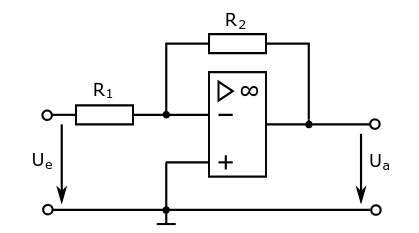
\includegraphics[width=0.4\textwidth]{images/invertierter_lin.png}%
                \caption{Das Schaltbild eines gegengekoppelten invertierten Linearverstärker. \cite{V51}}%
                \label{fig:invertierter_lin}%
            \end{figure}%
            \noindent
            Nach der Proportionalität der Ausgangsspannung zur Differenz der Eingangsspannungen gilt hier 
            \begin{equation}
                U_\text{N} = - \frac{U_\text{A}}{V}\, .
            \end{equation}
            Für den Knotenpunkt vor dem invertierten Eingang gilt bei $I_\text{N} = 0$ demnach 
            \begin{equation*}
                \frac{U_\text{N} - U_1}{U_\text{A} - U_1} = \frac{R_1}{R_1 + R_\text{N}}\, .
            \end{equation*}
            Hieraus folgt für die Verstärkung $V'$: 
            \begin{equation*}
                \frac{1}{V'} = - \frac{U_1}{U_\text{A}} = \frac{1}{V} + \frac{R_1}{R_\text{N}}\left(1 + \frac{1}{V}\right) \approx \frac{1}{V} + \frac{R_1}{R_\text{N}}\, ,
            \end{equation*}
            wobei die Näherung $V\gg 1$ genutzt wird. Es ist gut zu sehen, dass die Verstärkung bei $\frac{R_\text{N}}{R_1} \ll V$ quasi nur noch 
            von dem Verhältnis der Widerstände abhängig ist. 
            Da die Verstärkung $V$ stark schwanken kann, beispielsweise aufgrund der Temperatur, erhöht diese Gegenkopplung damit die Stabilität des Verstärkers. 
            Mit dem Faktor 
            \begin{equation*}
                g \coloneq \frac{V}{V'}
            \end{equation*}
            wird der Ausgangswiderstand verkleinert.
            Außerdem wird die Bandbreite um g erhöht, wie es in \autoref{fig:frequgang} zu sehen ist. 
            \begin{figure}[H]
                \centering
                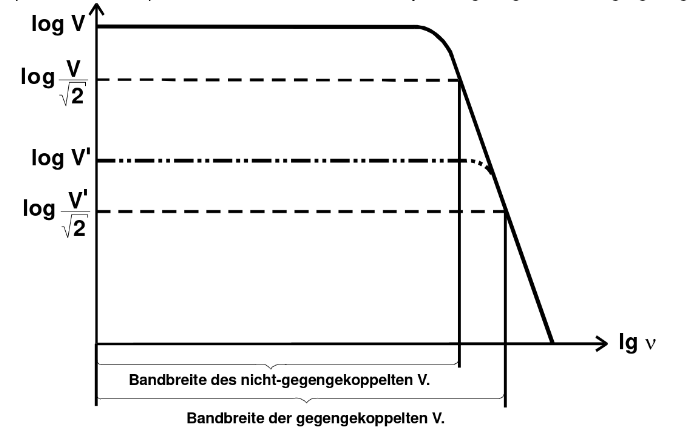
\includegraphics[width=0.6\textwidth]{images/frequenzgang_lin.png}
                \caption{Frequenzgang des Linearverstärkers. \cite{V51_old}}
                \label{fig:frequgang}
            \end{figure}

        \subsubsection{Umkehrintegrator}

            \noindent
            Ein Umkehrintegrator lässt sich wie in \autoref{fig:umkehrint} aufbauen.
            Hier ist unterschiedlich zum Invertierten Linearverstärker ein Kondensator in dem Rückkopplungszweig eingebaut.
            \begin{figure}[H]
                \centering
                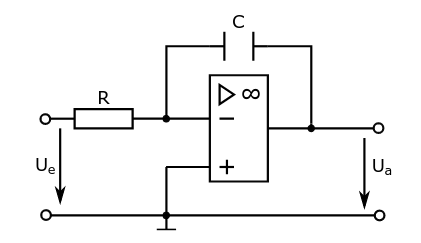
\includegraphics[width=0.4\textwidth]{images/Umkehrintegrator.png}
                \caption{Das Schaltbild eines Umkehrintegrators. \cite{V51}}
                \label{fig:umkehrint}
            \end{figure}
            \noindent
            Laut der Knotenregel ergibt sich für den Knotenpunkt vor dem invertierten Eingang 
            \begin{equation*}
                I_1 + I_\text{C} = 0\, ,
            \end{equation*}
            wobei hier schon $I_\text{N} = 0$ gesetzt wurde wegen der verschwindenden Spannung $U_\text{N}$. 
            Es gilt 
            \begin{align*}
                I_1 &= \frac{U_1}{R_1} \\ 
                \int I_\text{C} \, \text{d}t &= C U_\text{A}\, ,
            \end{align*}
            sodass sich die Ausgangsspannung zu 
            \begin{equation*}
                U_\text{A} = - \frac{1}{RC} \int U_1 \, \text{d}t
            \end{equation*}
            berechnet. 
            Die Ausgangsspannung ergibt sich also aus dem Integral der Eingangsspannung, welches den Namen der Schaltung motiviert. \\
            Für eine Eingangsspannung $U_1 = U_0 \sin(\omega t)$ folgt somit eine Ausgangsspannung 
            \begin{equation}
                U_\text{A} = \frac{U_0}{RC\omega} \cos(\omega t)\, .
                \label{eqn:int}
            \end{equation}

        \subsubsection{Invertierter Differenzierer}

            \noindent
            Ein invertierter Differenzierer ist in \autoref{fig:inverdiff} zu sehen. 
            Es ist zu erkennen, dass sich zum Umkehrintegrator nur die Platzierung des Widerstandes und des Kondensators vertauscht hat.
            \begin{figure}[H]
                \centering
                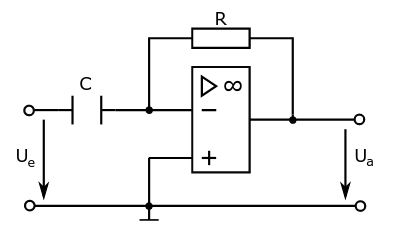
\includegraphics[width=0.4\textwidth]{images/invertierter_diff.png}
                \caption{Das Schaltbild eines invertierten Differenzierer. \cite{V51}}
                \label{fig:inverdiff}
            \end{figure}
            \noindent
            Die Knotenregel für den Knotenpunkt vor dem invertierten Eingang ergibt hier 
            \begin{equation*}
                I_1 + I_\text{A} = 0\, ,
            \end{equation*}
            wobei sich die einzelnen Ströme zu 
            \begin{align*}
                I_1 &= \dot{Q} = C \cdot \dot{U_1} \\
                I_\text{A} &= \frac{U_\text{A}}{I_\text{A}}
            \end{align*}
            ergeben. 
            Dadurch steht die Ausgangsspannung in einem Zusammenhang mit der zeitlichen Ableitung der Eingangsspannung
            \begin{equation*}
                U_\text{A} = - RC \cdot \dot{U_1}\, .
            \end{equation*}
            Für eine sinusförmige Eingangsspannung $U_1 = U_0 \sin(\omega t)$ ergibt sich dann eine Ausgangsspannung 
            \begin{equation}
                U_\text{A} = - R C U_0 \omega \cdot \cos(\omega t)\, ,
                \label{eqn:dif}
            \end{equation}
            welche eine lineare Proportionalität zur Frequenz hat.

        \subsubsection{Nichtinvertierter Schmitt-Trigger}

            \noindent 
            Bei dieser Schaltung wird die Ausgangsspannung über einen Widerstand in den nicht-invertierten Eingang des Operationsverstärkers gegeben.
            Dies ist in \autoref{fig:schmitttrig} visualisiert.
            \begin{figure}[H]
                \centering
                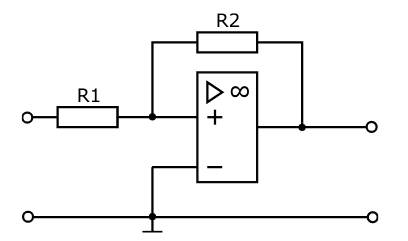
\includegraphics[width=0.4\textwidth]{images/schmitt_trigger.png}
                \caption{Das Schaltbild einer Schmitt-Triggerschaltung. \cite{V51}}
                \label{fig:schmitttrig}
            \end{figure}
            \noindent
            Es kommt somit zu einer Mitkopplung, ein größeres Ausgangssignal ergibt ein größeres Eingangssignal, sodass es ein recht instabiles Verhalten gibt 
            und die Ausgangsspannung sprungartig auf $\pm U_\text{S}$ geht, sobald die Eingangsspannung bestimmte Schwellenwerte erreicht. 
            Dies ist in \autoref{fig:abbschmitt} nochmal dargestellt. Das Ausgangssignal ist also eine Rechteckspannung.
            \begin{figure}[H]
                \centering
                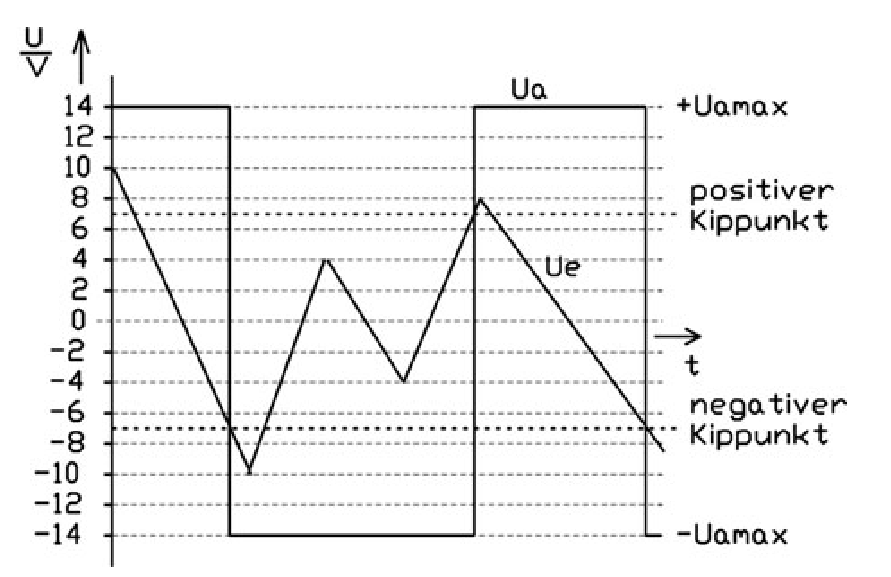
\includegraphics[width=0.4\textwidth]{images/schmitt_trig_dia.png}
                \caption{Ein $U_E$-$U_\text{A}$ Diagramm des Schmitt-Triggers. \cite{Joachim}}
                \label{fig:abbschmitt}
            \end{figure}
            Die Schwellwerte der Eingangsspannung lauten 
            \begin{align*}
                - \frac{R_1}{R_\text{P}} U_\text{S} && \text{und} && \frac{R_1}{R_\text{P}} U_\text{S} \, .
            \end{align*}

        \subsubsection{Signalgenerator}

            \noindent 
            Wird einen Schmitt-Trigger ein Umkehrintegrator nachgeschalten, wie es in \autoref{fig:signal} gezeichnet ist, so fängt das System spontan an zu 
            schwingen. 
            \begin{figure}[H]
                \centering
                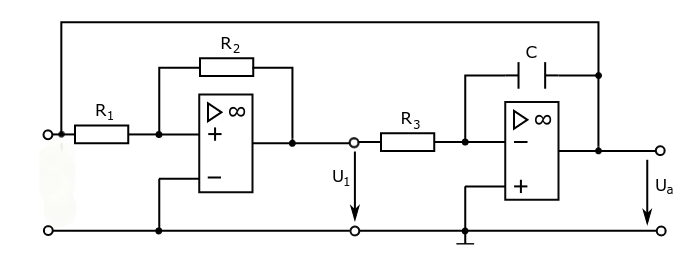
\includegraphics[width=0.8\textwidth]{images/signalgenerator.png}
                \caption{Das Schaltbild eines Signalgenerators. \cite{V51}}
                \label{fig:signal}
            \end{figure}
            \noindent
            Die konstante Spannung, die aus dem Schmitt-Trigger kommt, wird integriert. 
            Die Ausgangsspannung aus dem Umkehr-Integrator, wird als $U_1$ genutzt, sodass die Eingangsspannung des Schmitt-Triggers einen
            Schwellenwert erreicht. 
            In den Integrator wird eine konstante Spannung mit anderem Vorzeichen gegeben. 
            Insgesamt ergibt sich als Ausgangsspannung eine Dreiecksspannung mit 
            \begin{align*}
                \text{Frequenz}\, : & & \text{und} & & \text{Amplitude}\, :& \\
                \nu_\text{Dreieck} &= \frac{R_2}{4 C R_1 R_3} & & &A &=  U_\text{max} \frac{R_1}{R_2} \, .
            \end{align*}
